% !TeX root = ../main.tex
% Add the above to each chapter to make compiling the PDF easier in some editors.

\chapter{Development}\label{chapter:development}
With research done, the list of proposed features as well as the basic requirements and constraints of the tool had to be compiled into a sound implementation concept. As is usual and likely inevitable for development, changes had to be made over the course of the project and certain obstacles were hit, both covered in the latter two subsections of this chapter.

\section{Concept}
\paragraph{Technical constraints} Constraints presented through the platform the framework is to be built on are mostly bound to Unity engine. Since the Unity toolset only works on x86-based computers running Windows 7 or up or Mac OS X 10.8 or up and requires graphics hardware supporting DirectX 9 with shader model 3.0 or up \cite{SREQ}, the same applies for ConText. Since the source code for ConText is entirely written in C\#, code modification on Mac OS requires an IDE capable of handling C\# such as MonoDevelop. As Unity Technologies put it, "The rest mostly depends on the complexity of your projects", at least for the development system. Depending on the target platform the resulting game is ported to, additional constraints are the availability of the respective devices with sufficiently recent operating system versions.
\paragraph{Layers} With these underlying system requirements given, the ConText framework itself was envisioned as a layered construct with modular structure both internally and externally. Ideally, this would provide a high degree modularity and flexibility. 
The layered construct borrows an idea similar to that found in standardized system layer definitions with categories of actions and objects in the framework assigned to different layers, with communication or interfacing function calls happening between the layers. This would encapsulate and decouple similar functionality and make it easier to identify and modify or expand specific parts. The following layers are part of the concept:
\begin{enumerate}
\item The \textbf{Manager Layer} consists of all managers, which essentially represent the central logic handling the communication, tracking and updating of the game elements. The following managers are part of the Manager Layer:
	\begin{enumerate}
	\item The \textbf{Module Manager} which would keep track of all story modules in the storyline, provide functions for loading modules in or out, prompting the Log Manager to trigger log entries and the UI Manager to display modules in the game UI.
	\item The \textbf{UI Manager} would keep track of the UI objects for instanced story modules, handle scaling of the UI on the playing device and provide functions for displaying story modules, log entries and other info.
	\item The \textbf{Input Manager}, intended to handle (touch) input and redirect or trigger the according reactions to the respective affected managers.
	\item The \textbf{State Manager} which would handle saving and loading of story progress, keep track of the current game state and generally juggle the bits of data that don't fit into any of the other managers.
	\item The \textbf{Log Manager}, to keep track of all log entries and provide functions for loading and updating entries.
	\end{enumerate}
	The Input Manager would directly communicate with the Input Layer, the UI Manager with the UI Layer and the Module Manager with the Module Layer.
\item The \textbf{Input Layer} is very compact and only contains immediate input handling,  basically entirely computed by Unity's internal input handler. As such it might be seen as only a theoretical layer, or at least not an actual layer of ConText itself.
\item The \textbf{UI Layer} which contains the UI settings, visual ingame representations of the text/story module stream, the log list and a UI wrapper to channel calls and communication of the former to the UI Manager.
\item The \textbf{Modules Layer} is essentially the whole collection of modules and module instances and directly communicating the the Module Manager to exchange information about next modules and the storyline's elements.
\end{enumerate}
Where the layer concept actually differs somewhat from the usual definition of layers is that they don't communicate exclusively vertically. The Modules, Input and UI Layers all communicate with and via the Manager Layer.
\paragraph{Modules} The initial concept did not contain specific implementation details for the inner logic of individual parts, however the internal messages were defined as far as that they were to be designed as modules, with each module encapsulating one message and containing pointers to both the previous and next modules, akin to a double-linked list, the message data such as the respective sending character, the message content and a unique message ID and functions interfacing in a given way with the managers. 

As such, the user would be able to plug together the story with a list of these modules, or even expand the system with their own modules if they want specific functionality. It would only require them to implement the specific details of the interfacing functions to work in line with the module system. 

\begin{figure}[h]
\centering
\includegraphics[width=0.85\textwidth]{figures/concept.png}
\caption[Initial structural concept for ConText]{Initial structural concept for ConText.}\label{fig:concept}
\end{figure}

\paragraph{Editor interface} While the previous paragraphs specify the structure of the framework's systems and offerings, there was also considerations to be made for the interface provided to the developers and users. As ConText is a Unity plugin/package, it is informally bound to the established design used by Unity in order to be more accessible and seamlessly integrated into the engine during use. This mostly targets spatial arrangement and sizing of windows such as the inspectors and the ConText Options, as well to a degree the arrangement and design of controls within each window. For the initial concept, however, no specific constraints were yet set for the detailed presentation of information and as such started out as a vaguely ordered list of options and data controls.

\section{Final structure}
Regarding the final structure of the ConText framework an overview with consideration of the differences is presented first, followed by a more detailed look at perhaps the most central part, the message module system. 
\paragraph{Overview} For the development system used, the same technical constraints as with the concept are present, as Unity is still used for the tool. 
The layer structure is mostly retained with Input, Manager, Modules and UI Layers still in place, but communication between the layers is not as channeled as in the concept. Most calls from Input, Modules and UI still happen with and via the Managers layer, but both Input and UI layers also directly communicate with parts of the Modules layer. Thus there is no real distinction between horizontal and vertical layers and the structure is more akin to components in a graph than strict layers. As such one proposed change for a future revision would be to assess and rework the irregular communication between the components and decouple them in a more organized manner. 

The Manager Layer has seen the most drastic changes since the initial concept compared to the other layers. The Input Manager is removed entirely as the input is redirected straight to the UI manager and UI objects and state manager changes related to UI actions as well. The State manager concept was essentially split up into the State manager keeping track of the current game state and the Unify class holding references to all managers. It is proposed the two are merged into one class. Additionally, a Story Settings part was split out designed to hold data related to the story properties of the game, namely a list of characters with their respective properties as well as the default message sound and background track for the game. The Module layer calls directly to the Story settings to get relevant data instead of requesting the information through the Module manager. The Module manager retained most of its concept design with the only differences being that module loading and storing is now managed by itself entirely and does not communicate with the State manager and that the UI layer can restart the module stream once it is stopped (while the concept envisioned the Module manager to keep exclusive control over the module stream).

The Input layer is even more of a theoretical construct than in the concept, as it turned out that all relevant input handling is done entirely by Unity's internal systems. As such it is still a layer of the structure but not in any way part of the ConText code base.
In the UI layer the text stream and log reference are stripped from the final implementation as the UI manager accesses the objects contained within the two parts in the concept are now directly accessed by the UI manager. What remained are the UI wrapper which keeps references to some of the UI menu's controls and parts and handles transitions between the three main UI views, as well as the UI settings which adhering to its title keeps track of settings such as the mapping of message modules with their UI templates and of visual properties of the UI views and modules. 

The Modules layer is implemented almost entirely as envisioned in the concept, with the small difference that the unique message ID is constructed from multiple partial IDs instead of one single number.

\begin{figure}[h]
\centering
\includegraphics[width=0.85\textwidth]{figures/final.png}
\caption[Final structure for ConText]{Final structure for ConText (low level details omitted). Visibly less clean than the initial concept.}\label{fig:final}
\end{figure}

\begin{figure}[h]
\centering
\includegraphics[width=0.85\textwidth]{figures/conceptVSfinal.png}
\caption[Layer comm. comparison concept vs final]{Comparison of the layer intercommunication between the two design stages. Note that the final structure more resembles vertical and horizontal component communication instead of strictly layers.}\label{fig:layerConceptVSFinal}
\end{figure}

\paragraph{Module system} The module system is by far not the only complex part of ConText, but it is certainly the most central part. As mentioned before, the story is made up of modules, which each encapsulate a message of some sort. As the game should be able to offer not just text, but perhaps also images or sounds to keep up a sense of variety, so the message modules have the following structure:
\begin{enumerate}
\item The \textbf{previous module}, which will always have been fired right before the current
\item The \textbf{message ID}, made up of four parts
	\begin{enumerate}
	\item A \textit{sequential part}, which denotes the message's sequential ID within its branch, 
	\item A \textit{branch part} denoting the branch the message is in, respective to the latest prior module with multiple outgoing connections, 
	\item A \textit{hierarchy part} representing the hierarchy level of the message, with the hierarchy increasing for each branching module, 
	\item A \textit{subpart ID} which is only calculated internally when the message has to be split up into multiple partial instances.
	\end{enumerate}
	With this structure, each message has its unique identifier. The hierarchy part first specifies which level the message is on, after which branch split it follows, the branch part specifies which of the split branches it lies in, the sequential part then specifies which in line it is in that branch, and the subpart part specifies another order when split partial messages between two consecutive sequential messages happen.
\item The \textbf{sending character} as in the character the message belongs to. The character does not need to be an actual person of the story if the message is not to be sent as a message in the visually classical sense, for example one might call the character "Narrative" or not give it any name and set the message property to disregard alignment in order to display it more like a simple text field.
\item The \textbf{message send delay} or \textbf{delay before send} in seconds which specifies how long the automatic stream should wait before deploying the message.
\item The \textbf{message sound}, not to be mistaken with the default message sound in the Story Settings. The latter is a sound played every time a message is triggered, the former is only played for this specific message and could for example be used to imitate a voice message.
\item The \textbf{message content} which is fully dependent on the message or rather module type. Default included in the framework are modules of with the content types \textbf{Text}, \textbf{Image}, both self-explanatory, as well as \textbf{Tic Tac Toe} to show how a mini game may be used to provide more involved gameplay to the user and \textbf{Reply} which provides the player with several choices to reply to a message and can be used to query knowledge, opinions an direct the story along different paths. These types specify which form of content can be set. - Note: text content can include a simple markup command that will split up the text portion of the module into multiple messages with the respective specified delay. 
\item The \textbf{log entry} which may contain additional information not fit for the message itself and which can then be viewed in the Log view.
\item The \textbf{next module} analogously to the previous module specifying which module comes next. Depending on the module type, there can be multiple next modules, such as with the Reply module. To note here is that implementation is subpar as a single next module is part of the basic module type, but multiple next modules are additions made only to the code of branching modules. A proposed change is that next modules be a list with variable length in order to enable better compatibility with calls working with next module data.
\end{enumerate}

\begin{figure}[h]
\centering
\includegraphics[width=0.4\textwidth]{figures/msgmod.png}
\caption[Message module structure]{The common structure of a ConText message module.}\label{fig:msgmod}
\end{figure}

The communication procedure for message modules is best explained through an example. Assumed be the following parameters: 
\begin{enumerate}
\item The framework is correctly configured. 
\item The story consists of the modules 
	\begin{enumerate}
	\item M1-T of type Text Module, 
	\item M2-R of type Reply Module and 
	\item three Mi-T of type Text Module with 3 <= i <= 5, 
	\end{enumerate}
with M2-R being the successor to M1-T and M3-T, M4-T and M5-T as the replies outgoing from M2-R. 
\item Playback starts with M1-T as the first story module.
\end{enumerate}

\begin{figure}[h]
\centering
\includegraphics[width=0.7\textwidth]{figures/sampleStory.png}
\caption[Sample story structure]{The sample story structure.}\label{fig:smpstory}
\end{figure}

As shown in figure \ref{fig:loop1} once the story playback is started, the module manager will initiate the automatic text stream. As the first module is specified as M1-T, the manager will access M1-T to grab the sending delay and message sounds to delay the message firing accordingly and trigger the sound. Then it will pass the module object to the UI manager for instancing. 
The UI manager attempts to find the correct UI template mapping for M1-T's type and instance a GameObject using the template. Next the module's setContent function will be called with the template instance as a parameter in order to input its specific message info into the UI instance. The details of this are down to the specific type, but for the case of M1-T, the setContent function will put the message's sender and message send time at the top of the message bubble, the message text as the main text portion and adjust width and side padding for correct alignment, quite like a text bubble in a common messenger app. Once the content is set, the UI manager takes over again and adds the instance into the Text View's scroll area, scrolls to the bottom to make the new module the latest displayed and finally adds the instance to the module manager's list of instanced messages.
At this point, control is returned to the module manager. With M1-T's instancing completed, the automatic stream attempts to grab the next module in line via the getNextPart function implemented in each module type's class. This will return whichever module is set as the next module or a null return. When null is returned, the automatic stream will stop and be halted until something starts it again, such as specific user input. In M1-T's case, the call will return M2-R. 

\begin{figure}[H]
\centering
\includegraphics[width=\textwidth]{figures/sampleStep1.png}
\caption[First mod. sys. loop iteration]{The first loop iteration of the automatic stream. M1-T is instanced, filled with content, then the next module is acquired, starting the second loop iteration.}\label{fig:loop1}
\end{figure}

See figure \ref{fig:loop2}, the automatic text stream's loop starts from the top again, computing M2-R's UI template mapping, waiting the send delay, playing the message sound and handing over the module to the UI manager. Once the content is set for M2-R, the module manager will again request the next module. This time the call will return null as the Reply module offers reply choices to the player and does not know the next module until the player has made a choice. Once the player chooses an option, the corresponding option will call the restart function of the module manager which will continue the automatic stream with the now known next module. 
As such, the stream loop will again start from the top with M3-T, M4-T or M5-T. 
A similar system is used when loading previously saved story progress, excluding any sending delays or user input interrupts. 

\begin{figure}[H]
\centering
\includegraphics[width=\textwidth]{figures/sampleStep2.png}
\caption[Second mod. sys. loop iteration]{The second loop iteration of the automatic stream. M2-R is instanced, filled with content, then the next module is "null" as the outcome is not known yet, halting the automatic stream. Only once user input happens and a reply is chosen, the next module is known, starting the third loop iteration.}\label{fig:loop2}
\end{figure}

\paragraph{Editor interface} Through reiteration, user feedback, user experience and usability research, the editor interface was transformed from the continuously grown messy list of data controls and options in some of the ConText windows to a more clean looking appearance with logical order and structuring and visual decoupling as well as hiding and layered display to reduce the visible clutter and complexity.

\begin{figure}[H]
\centering
\includegraphics[width=0.9\textwidth]{figures/inengineSample_rot.png}
\caption[Inengine view and layout]{The image presented by the framework in its current state, with the story graph opened separately. (rotated for readability)}\label{fig:editor}
\end{figure}
\begin{figure}[H]
\centering
\includegraphics[width=0.6\textwidth]{figures/inengineStory.png}
\caption[Inengine story sample]{A brief story put together in ConText and run in preview mode.}\label{fig:inengineStory}
\end{figure}

\section{Stumbling blocks}
Along the way, development of ConText stumbled across a few difficulties, posed by discrepancies between the concept and expected implementation versus the viable possibilities offered through Unity as well as general concept insufficiency. 
\paragraph{Game UI} The UI for games created with the framework use the "new" UI system introduced with Unity 4.6 and Unity 5.0, which is based on canvas-object relationships, full material supported texture drawing and internally managed screen space dependent scaling and alignment instead of the previously used low level primitive drawing functions. This allows for easier creation of complex and detailed user interfaces but also poses new constraints when using higher level features of the system such as automated alignment or ordering, the latter of which turned out to be a longer running hassle to get working right. Specifically, the module stream should eventually automatically display the modules in correct order, correct scaling and allow the user to scroll through them, with correct scaling being the crux here. The UI system offers settings and components for measurement limits and dependencies, but at first sight is inconsistent in how it applies them across GameObjects and even object types. Hierarchical structures need to be set up in a more complex and unintuitive way to get the scaling of low level items working right and based on their content. A solution was found on the Unity3D forums eventually, along with a reply by a Unity Technologies employee indicating the UI system was designed with certain such drawbacks known but accepted for performance and simplicity concerns \cite{U3DC1}. The alternative to this solution would have been to create a custom approximation for message module scaling, requiring a lot more time and likely increasing complexity of module code.
\paragraph{Inspector heritage} Another problem encountered is mostly to be attributed to subpar planning and vague concept design. The initial concept did not consider the number of interfacing functions the module classes and their editor inspectors would require, and as such first implementation only had a select few calls integrated into the parent class to all module inspector types. It was not until close to the project deadline that a major refactoring attempt was made and many parts of the respective classes were centralized into the highest parent, eliminating the majority of duplicated module inspector code and reducing the respective code files' footprint by more than half. Similar happened on a smaller scale to the module classes throughout the project as well. It is proposed a more ideal modification would be to use a custom defined interface for both module types and module inspectors instead of the simple parent structure employed in the current revision of the framework. This would make sure experienced users implement all necessary functions for custom module types and would also simplify possible future extensions. 
\paragraph{User study} When conducting the two user studies of this thesis, there were severe problems with finding participants and receiving sufficient feedback to the surveys. This problem is discussed in more detail in sections 4.2 and 4.3. 